\section{Dynamic Power Reactor}
\label{sec:dpr_method}

The \gls{nrc} publishes a daily Power Reactor Status report for each reactor
under its jurisdiction \cite{nrc_power_2025}. These reports contain, amongst
other things, the percentage of the total power capacity at which the operators
say the reactor operated. In the case of a fuel cycle simulation containing a
small number of reactors or a full fleet simulation over a short time, the
differences in the power predicted by the \cycamore reactor and reality can
diverge.

In Figure \ref{fig:pp_full} we examine the single reactor operating at the
\gls{clinton}, with a reference unit power capacity (i.e., net power) of 1062
MWe according to the \gls{iaea} \gls{pris} database \cite{IAEA_PRIS}, and
compare it to the results from the \cycamore reactor modeled over the same time
frame. This figure excludes the startup of the \cycamore reactor, which we set
several months before this window to ensure that it was operating on the same
schedule as the data from the \gls{nrc} suggest the real reactor was operating
from the start of 2021 through the end of 2024.

\begin{figure}[H]
  \centering
  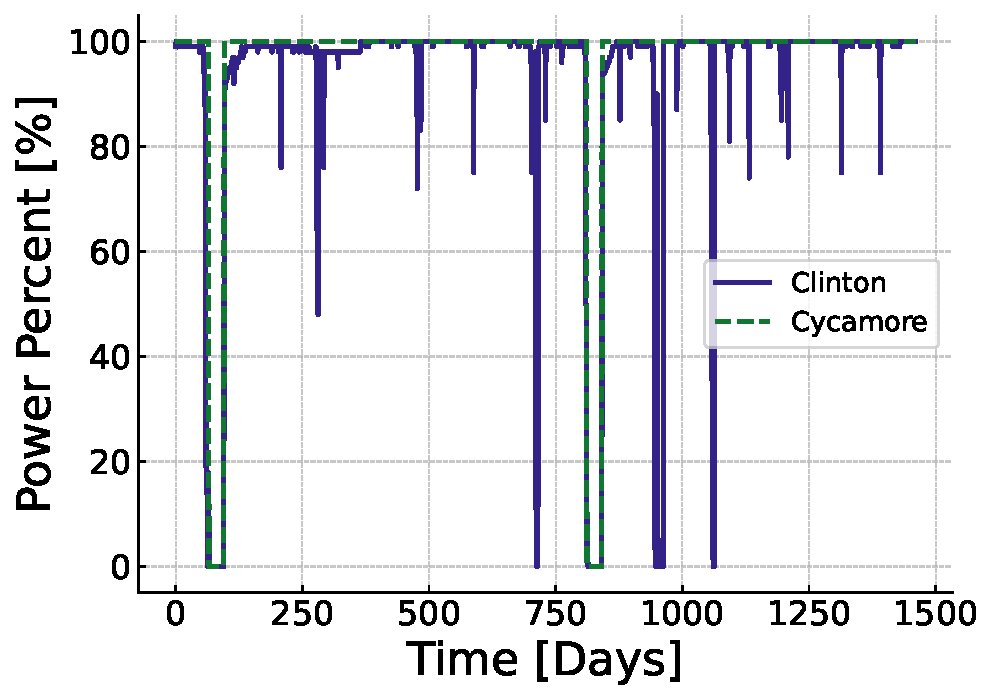
\includegraphics[width=0.7\linewidth]{images/power_reactor/power_percent_clinton_fake.pdf}
  \caption{\gls{clinton} reactor daily power percent 2021-2024}
  \label{fig:pp_full}
\end{figure}

Performing a simple numerical integration, we find that the total energy
produced by both reactors differ by just under 51 GWe with a percent difference
of 3.52\%. This difference can be negated by comparing it to a base case, but
for our small-scale model, users might be interested in incorporating realistic
fluctuations in power and find that the two scenarios in Figure
\ref{fig:pp_full} were not equal on 908 days, or 62.2\%, of the 1460-day
simulation. For this work, we introduce the \gls{dpr} to mirror this
variability in power we see in Figure \ref{fig:pp_full}. \gls{dpr} functions
the same way as the \cycamore reactor, except the user can input the percentage
of the total power capacity the reactor is outputting at any given time step.


\begin{figure}[H]
  \centering
  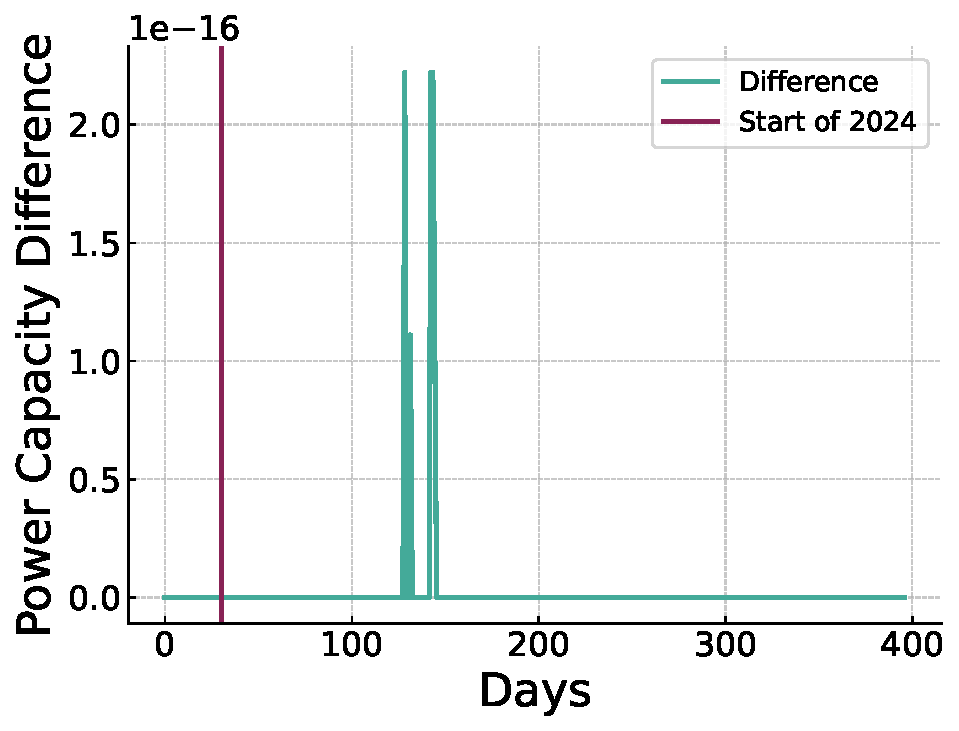
\includegraphics[width=0.7\linewidth]{images/power_reactor/dpr_diff.pdf}
  \caption{Difference in daily power capacity between \gls{dpr} and \gls{clinton}.}
  \label{fig:dpr_clinton_diff}
\end{figure}


If we narrow the scope of this study to 2024, Figure \ref{fig:dpr_clinton_diff}
shows how \gls{dpr} replicates the real power capacity fluctuations with the
difference between the reported values from the \gls{nrc} \cite{nrc_power_2025}
and the results from our \cyclus simulation. The maximum difference between the
two is $2.22 \times 10^{-16}$, which is explainable by floating point error in
calculations as this value matches a double point machine epsilon value. Figure
\ref{fig:dpr_cycamore_power} compares \gls{dpr} to the \cycamore reactor. As
the reactors are assumed to start operations before 2024, we have added a
buffer month in which the reactors fuel. We indicate, with a vertical line,
when 2024 begins to show the period over which we compare the results from
\cyclus.


\begin{figure}[H]
  \centering
  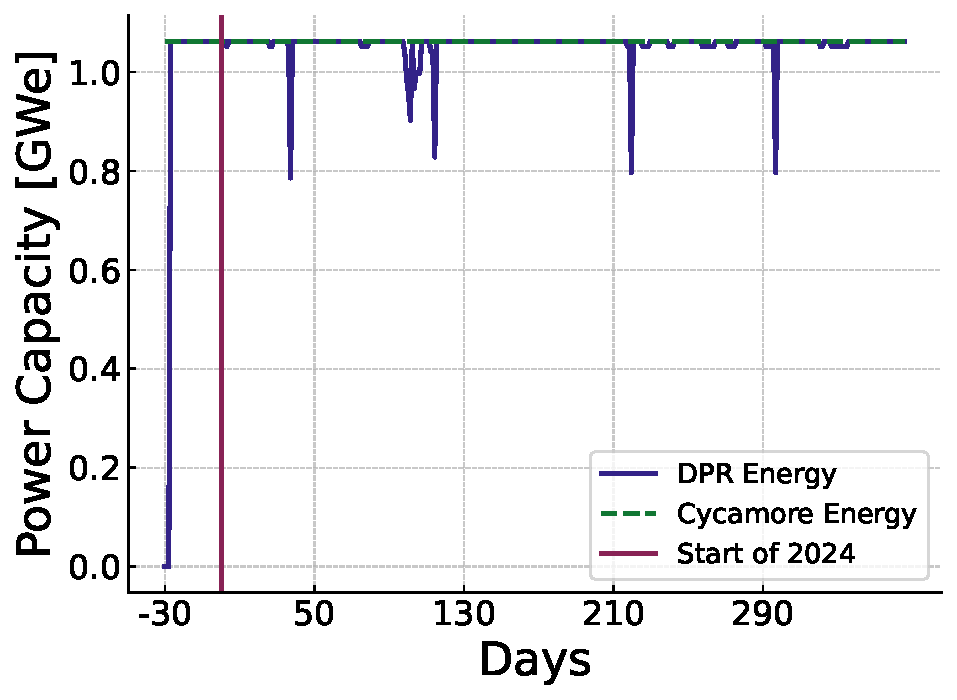
\includegraphics[width=0.7\linewidth]{images/power_reactor/dpr_cycamore_energy.pdf}
  \caption{2024 power capacity of the \cycamore reactor and \gls{dpr}.}
  \label{fig:dpr_cycamore_power}
\end{figure}


